\documentclass[twoside,11pt,a4paper]{article}
 
\usepackage[utf8]{inputenc}
\usepackage{amsmath, amssymb, latexsym}
\usepackage{sidecap}
 
\usepackage{tikz}
\usetikzlibrary{decorations.pathreplacing}
\usepackage[colorinlistoftodos, color=green!40, prependcaption]{todonotes}
\usepackage{booktabs}
\usepackage{comment}
\usetikzlibrary{positioning,chains}
\usepackage{tikz}
\usepackage{lipsum,adjustbox}
\usepackage{empheq} 
\usetikzlibrary{shapes,arrows,positioning}
\usetikzlibrary{fit, arrows.meta, shapes}
\usetikzlibrary{external}
\tikzexternalize % activate!
\newcommand{\subsubsubsection}[1]{\paragraph{#1}\mbox{}\\}
\setcounter{secnumdepth}{4}
\setcounter{tocdepth}{4}

\mathtoolsset{showonlyrefs=false} 
\usepackage{xcolor}
\usepackage{hyperref} % For hyperlinks in the PDF
%\setlength{\marginparwidth}{2.5cm}
\bibliographystyle{apsrev4-1}
%\bibliographystyle{apalike}
\usepackage{tikz}
\usetikzlibrary{quantikz}
% defines the color of hyperref objects
% Blending two colors:  blue!80!black  =  .8 blue and 0.2 black       % automagic cross-referencing
\hypersetup{ % this is just my personal choice, feel free to change things
    colorlinks,
    linkcolor={red!50!black},
    citecolor={blue!50!black},
    urlcolor={blue!80!black}}

\usepackage{listings}
\lstset{language=C, keywordstyle={\bfseries \color{blue}}}

\bibliographystyle{apsrev4-1}




\begin{document}


\begin{figure}
    \centering
    
\newcommand{\empt}[2]{$#1^{\langle #2 \rangle}$}

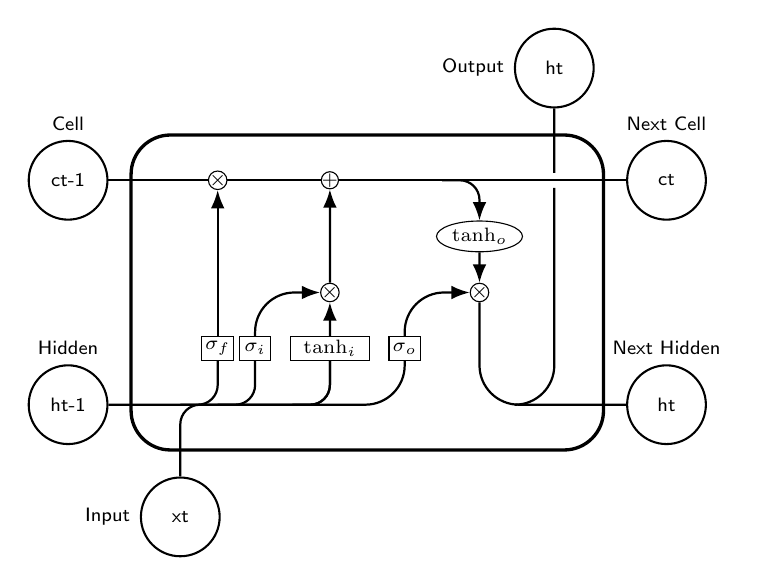
\begin{tikzpicture}[scale=0.95,
    % GLOBAL CFG
    font=\sf \scriptsize,
    >=LaTeX,
    % Styles
    cell/.style={% For the main box
        rectangle, 
        rounded corners=5mm, 
        draw,
        very thick,
        },
    operator/.style={%For operators like +  and  x
        circle,
        draw,
        inner sep=-0.5pt,
        minimum height =.2cm,
        },
    function/.style={%For functions
        ellipse,
        draw,
        inner sep=1pt
        },
    ct/.style={% For external inputs and outputs
        circle,
        draw,
        line width = .75pt,
        minimum width=1cm,
        inner sep=1pt,
        },
    gt/.style={% For internal inputs
        rectangle,
        draw,
        minimum width=4mm,
        minimum height=3mm,
        inner sep=1pt
        },
    mylabel/.style={% something new that I have learned
        font=\scriptsize\sffamily
        },
    ArrowC1/.style={% Arrows with rounded corners
        rounded corners=.25cm,
        thick,
        },
    ArrowC2/.style={% Arrows with big rounded corners
        rounded corners=.5cm,
        thick,
        },
    ]

%Start drawing the thing...    
    % Draw the cell: 
    \node [cell, minimum height =4cm, minimum width=6cm] at (0,0){} ;

    % Draw inputs named ibox#
    \node [gt] (ibox1) at (-2,-0.75) {$\sigma_f$};
    \node [gt] (ibox2) at (-1.5,-0.75) {$\sigma_i$};
    \node [gt, minimum width=1cm] (ibox3) at (-0.5,-0.75) {$\tanh_i$};
    \node [gt] (ibox4) at (0.5,-0.75) {$\sigma_o$};

   % Draw opérators   named mux# , add# and func#
    \node [operator] (mux1) at (-2,1.5) {$\times$};
    \node [operator] (add1) at (-0.5,1.5) {+};
    \node [operator] (mux2) at (-0.5,0) {$\times$};
    \node [operator] (mux3) at (1.5,0) {$\times$};
    \node [function] (func1) at (1.5,0.75) {$\tanh_o$};

    % Draw External inputs? named as basis c,h,x
    \node[ct, label={[mylabel]Cell}] (c) at (-4,1.5) {\empt{c}{t-1}};
    \node[ct, label={[mylabel]Hidden}] (h) at (-4,-1.5) {\empt{h}{t-1}};
    \node[ct, label={[mylabel]left:Input}] (x) at (-2.5,-3) {\empt{x}{t}};

    % Draw External outputs? named as basis c2,h2,x2
    \node[ct, label={[mylabel]Next Cell}] (c2) at (4,1.5) {\empt{c}{t}};
    \node[ct, label={[mylabel]Next Hidden}] (h2) at (4,-1.5) {\empt{h}{t}};
    \node[ct, label={[mylabel]left:Output}] (x2) at (2.5,3) {\empt{h}{t}};

% Start connecting all.
    %Intersections and displacements are used. 
    % Drawing arrows    
    \draw [ArrowC1] (c) -- (mux1) -- (add1) -- (c2);

    % Inputs
    \draw [ArrowC2] (h) -| (ibox4);
    \draw [ArrowC1] (h -| ibox1)++(-0.5,0) -| (ibox1); 
    \draw [ArrowC1] (h -| ibox2)++(-0.5,0) -| (ibox2);
    \draw [ArrowC1] (h -| ibox3)++(-0.5,0) -| (ibox3);
    \draw [ArrowC1] (x) -- (x |- h)-| (ibox3);

    % Internal
    \draw [->, ArrowC2] (ibox1) -- (mux1);
    \draw [->, ArrowC2] (ibox2) |- (mux2);
    \draw [->, ArrowC2] (ibox3) -- (mux2);
    \draw [->, ArrowC2] (ibox4) |- (mux3);
    \draw [->, ArrowC2] (mux2) -- (add1);
    \draw [->, ArrowC1] (add1 -| func1)++(-0.5,0) -| (func1);
    \draw [->, ArrowC2] (func1) -- (mux3);

    %Outputs
    \draw [-, ArrowC2] (mux3) |- (h2);
    \draw (c2 -| x2) ++(0,-0.1) coordinate (i1);
    \draw [-, ArrowC2] (h2 -| x2)++(-0.5,0) -| (i1);
    \draw [-, ArrowC2] (i1)++(0,0.2) -- (x2);

\end{tikzpicture}

\end{figure}


\end{document}


